\documentclass[10pt]{article}

\usepackage[letterpaper,margin=0.86in]{geometry}
\usepackage{amsmath,amssymb,amsthm,mathtools}
\usepackage{booktabs,tabularx,array,multirow}
\usepackage{microtype}
\usepackage{enumitem}
\usepackage{listings}
\usepackage{xcolor}
\usepackage{hyperref}
\usepackage{url}
\usepackage{fancyhdr}
\usepackage{graphicx}
\usepackage{float}
\usepackage{tikz}
\usetikzlibrary{arrows.meta,positioning,fit}

\definecolor{accent}{HTML}{234A73}
\definecolor{soft}{HTML}{F4F6F8}
\definecolor{rulegray}{HTML}{D7DCE2}
\hypersetup{colorlinks=true,linkcolor=accent,citecolor=accent,urlcolor=accent,pdftitle={Operator-Level Boolean Computation with Correspondence Matrices},pdfauthor={Brian Theory}}
\setlength{\parindent}{1.05em}
\setlength{\parskip}{0pt}
\setlist{nosep,leftmargin=*}
\pagestyle{fancy}
\fancyhf{}
\fancyhead[L]{\small Operator-Level Boolean Computation with Correspondence Matrices}
\fancyhead[R]{\small Post-split revised compiler draft}
\fancyfoot[C]{\thepage}
\setlength{\headheight}{14pt}
\emergencystretch=2em

\newcommand{\B}{\mathbb B}
\newcommand{\Ftwo}{\mathbb F_2}
\newcommand{\bxor}{\mathbin{\Updownarrow}}
\newcommand{\ptop}[1]{\widehat{#1}}
\newcommand{\Pair}{\operatorname{Pair}}
\newcommand{\supp}{\operatorname{supp}}
\newcommand{\eval}{\mathcal E}
\newcommand{\IR}{\mathrm{IR}}
\newcommand{\AST}{\mathrm{AST}}
\newcommand{\true}{\mathrm{T}}
\newcommand{\false}{\mathrm{F}}

\theoremstyle{plain}
\newtheorem{theorem}{Theorem}
\newtheorem{lemma}{Lemma}
\newtheorem{proposition}{Proposition}
\theoremstyle{definition}
\newtheorem{definition}{Definition}
\theoremstyle{remark}
\newtheorem{remark}{Remark}

\lstset{
  basicstyle=\ttfamily\small,
  backgroundcolor=\color{soft},
  frame=single,
  rulecolor=\color{rulegray},
  columns=fullflexible,
  keepspaces=true,
  breaklines=true,
  xleftmargin=0.5em,
  xrightmargin=0.5em,
  aboveskip=0.7em,
  belowskip=0.7em
}

\title{\vspace{-1.3em}\textbf{Operator-Level Boolean Computation with Correspondence Matrices}\\[0.35em]
\large Typed operand frames, local operator folding, fallback semantics, and empirical boundaries}
\author{Brian Theory}
\date{Post-split revised computational draft --- 22 September 2026}

\begin{document}
\maketitle

\begin{abstract}
Correspondence matrices (CMs) encode a binary Boolean connective as a four-bit $2\times2$ operator in a declared operand frame. This paper studies a compiler transformation built on that representation rather than claiming a new truth-table algebra. The compiler recognizes binary operator occurrences, records their row/column operands and polarities, transports swapped or negated occurrences into a canonical frame, and fuses tokens only after exact frame agreement. It distinguishes pure structural folding, hybrid folding through locally retabulated descendants, whole-root four-assignment retabulation, and ordinary fallback. We state a common semantic invariant and prove soundness for each admitted pair path. The implementation keeps compact tokens, framed pair surrogates, general Boolean IR, lowered programs, and dense outputs as distinct artifacts so that constant-size kernel operations are not confused with end-to-end costs. Existing exploratory S1/S2 records show that local small-function folding can reduce pre-expansion work in some strata, but a matched generic local truth-function optimizer reaches the same reduced outputs. A separately frozen ANF-dispatch study is negative overall: highly profitable selected synthetic folds do not repay dispatcher overhead on the aggregate synthetic and natural corpora. Broader current-source project benchmarks likewise emphasize task matching and strong packed/CSE controls, but they measure different endpoints and are not pair-compiler results. The confirmatory pair-compiler protocol against direct packed, prepared DAG, ROBDD, and synthesis-compatible baselines remains unexecuted. The contribution is therefore a typed frame-aware compilation rule, its sound fallback boundary, and a disciplined evaluation framework for determining when local folding amortizes in practice.
\end{abstract}

\noindent\textbf{Draft status.} This is the revised compiler-focused manuscript after the deliberate CM/LM publication split. The companion foundations paper \emph{Correspondence and Logical Matrices: A Boolean Operator Calculus} owns the formula-valued LM theory, valuation, logical pairing, higher-arity tensors/maps, and the broader coherence calculus \cite{TheoryFoundations2026}. The present paper imports only the numeric binary contract required by the compiler. Protocol v3 has not yet been executed; no pair-compiler end-to-end speedup is claimed.

\section{Introduction and claim boundary}

A binary Boolean connective contains four output values. A correspondence matrix stores those four values as a $2\times2$ array whose row and column axes are tied to declared operands. In isolation, that is only a reshaping of a truth table. The computational question is different: can a compiler use the small operator as a first-class token, normalize the token's operand frame, and combine compatible local operators before evaluating or expanding their operands?

The key example is deliberately simple. Consider
\begin{equation}
 (X\Rightarrow Y)\bxor(Y\Rightarrow X).
 \label{eq:mismatch-expression}
\end{equation}
Both inner connectives are implication, but they do not initially refer to the same ordered operand frame. Treating their four-bit arrays as if corresponding entries described the same assignment would be a type error. Once the second occurrence is transported from frame $(Y,X)$ to frame $(X,Y)$ by transpose, entrywise XOR is sound:
\begin{equation}
 [\Rightarrow]\,\ptop{\bxor}\,[\Rightarrow]^T=[\bxor].
 \label{eq:mismatch-fold}
\end{equation}
The resulting token represents $X\bxor Y$. Equation~\eqref{eq:mismatch-fold} is not important because XOR of two truth tables is difficult; it is important because it makes the \emph{admission condition} explicit. A local table may be fused only when its coordinates have a common logical meaning.

This paper therefore treats operand-frame metadata as part of the compiler type. A successful pair compilation returns not just four bits, but a token tied to canonical row and column operands. Swaps and input polarities are normalized by fixed reindexings. Compatible tokens can then be fused by an outer Boolean connective before repeated operand work or polynomial expansion. If structural recognition fails, the implementation can exactly retabulate an admitted two-variable subtree, can combine such a retabulated descendant with structural parents while marking the result hybrid, or can leave the expression on the ordinary IR path.

The component operations have substantial prior art. Boolean matrices predate this work \cite{Edwards1972}; matrix and vector logics represent logical operators algebraically \cite{Stern1988,Mizraji1992,Mizraji2008}; Cheng, Zhao, and Xu explicitly combine truth vectors entrywise under an arbitrary outer Boolean operation \cite{Cheng2011}; small truth functions, NPN transformations, LUTs, and DAG-aware rewriting are standard synthesis techniques \cite{Mishchenko2006,Zhou2019,Testa2019}; and bit-parallel evaluators compute several assignments simultaneously \cite{Lee2022}. Bricken's internally dated 1997 technical note is also a close antecedent for $2\times2$ logical matrices and bra--matrix--ket evaluation \cite{Bricken1997}. The present paper does not claim those ingredients as new.

The narrower contribution is computational and testable:
\begin{enumerate}
  \item a \textbf{typed frame-aware compiler rule} in which a four-bit CM token is paired with operand metadata and normalized before same-frame fusion;
  \item \textbf{sound multi-path semantics} separating pure structural compilation, local retabulation, hybrid composition, and ordinary fallback;
  \item an \textbf{implementation and cost boundary} separating compact tokens, framed surrogates, general IR, lowered programs, and dense materialized outputs;
  \item \textbf{matched mechanism and negative evidence}: exploratory folding can reduce pre-expansion work, an equally capable generic optimizer can reproduce the same reductions, and a frozen dispatcher study shows that local wins need not amortize; and
  \item a \textbf{confirmatory methodology} that requires direct packed and sharing-aware comparators, preparation costs, reuse, output equivalence, memory, fallback, and failures to be measured on the same task.
\end{enumerate}

The scientific claim does not depend on CM folding being uniquely capable of a reduction. If a generic local truth-function optimizer reaches the same reduced form, that locates the mechanism in a broader family of small-function rewrites. The remaining CM-specific question is whether the representation and its frame metadata make recognition, legality, transformation, caching, or reuse sufficiently direct and inexpensive to matter in a full compiler.

\section{Minimal CM compiler contract}
\label{sec:minimal-contract}

The companion foundations paper develops the CM/LM calculus in detail \cite{TheoryFoundations2026}. Only the following binary numeric contract is required here.

Let
\begin{equation}
 \B=\{0,1\}\cong\Ftwo,
\end{equation}
with multiplication interpreted as conjunction and addition written as XOR, $\bxor$. For a bit $x\in\B$, use the true-first state
\begin{equation}
 |x\rangle=\begin{bmatrix}x\\ \neg x\end{bmatrix},
 \qquad
 \langle x|=\begin{bmatrix}x&\neg x\end{bmatrix}.
 \label{eq:state}
\end{equation}
For a binary logical connective variable $\Theta$, define the compact correspondence matrix
\begin{equation}
 [\Theta]
 :=
 \begin{bmatrix}
  \Theta_{11}&\Theta_{10}\\
  \Theta_{01}&\Theta_{00}
 \end{bmatrix}
 =
 \begin{bmatrix}
  1\Theta1&1\Theta0\\
  0\Theta1&0\Theta0
 \end{bmatrix}.
 \label{eq:cm}
\end{equation}
The row and column assignment order $(1,0)$ is part of the representation contract.

For $C\in\B^{2\times2}$, define the XOR--AND contraction
\begin{equation}
 \eval_C(x,y)=\langle x|C|y\rangle
 =\mathop{\bxor}_{r,s\in\{1,0\}}
 \chi_x(r)\wedge C_{rs}\wedge\chi_y(s),
 \label{eq:contraction}
\end{equation}
where $\chi_x(r)=1$ exactly when $r=x$.

\begin{proposition}[Selection]
For every binary connective $\Theta$ and $x,y\in\B$,
\begin{equation}
 \langle x|[\Theta]|y\rangle=x\Theta y.
 \label{eq:selection}
\end{equation}
\end{proposition}

\begin{proof}
Both states are one-hot. Every term in Equation~\eqref{eq:contraction} vanishes except the term at $(r,s)=(x,y)$.
\end{proof}

The compiler packs the four coefficients into a constant-size token. That token is not by itself sufficient to authorize a rewrite. An occurrence is also typed by an \emph{operand frame}: the row expression, column expression, their signed polarities, and the truth-state order. In the implementation considered here, a successful pair surrogate ultimately records canonical row and column variable names together with the normalized token.

\section{Typed normalization and same-frame fusion}
\label{sec:alignment}

Let
\begin{equation}
 P=\begin{bmatrix}0&1\\1&0\end{bmatrix}=[\bxor].
\end{equation}
Define $\Theta^\tau(x,y):=y\Theta x$. With the true-first convention,
\begin{align}
 [\Theta^\tau]&=[\Theta]^T, \\
 [\Theta(\neg X,Y)]&=P[\Theta], \\
 [\Theta(X,\neg Y)]&=[\Theta]P,
 \label{eq:input-transforms}
\end{align}
where products with $P$ are XOR--AND products and therefore act as row/column permutations. Output negation is entrywise complement.

For a binary outer connective $\Phi$, define same-position fusion by
\begin{equation}
 \bigl([\Theta_1]\ptop{\Phi}[\Theta_2]\bigr)_{rs}
 :=(\Theta_1)_{rs}\Phi(\Theta_2)_{rs}.
 \label{eq:pointwise}
\end{equation}
This is not matrix multiplication.

\begin{theorem}[Same-frame fusion]
If $[\Theta_1]$ and $[\Theta_2]$ are expressed in the same ordered operand frame, then for all $x,y\in\B$,
\begin{equation}
 (x\Theta_1 y)\Phi(x\Theta_2 y)
 =\left\langle x\middle|
 \left([\Theta_1]\ptop{\Phi}[\Theta_2]\right)
 \middle|y\right\rangle.
 \label{eq:fusion-theorem}
\end{equation}
\end{theorem}

\begin{proof}
Both sides select position $(x,y)$; the right-hand side stores the outer operation on exactly those two selected coefficients. No distributive law for $\Phi$ over XOR is required.
\end{proof}

The pointwise identity itself is classical; Cheng, Zhao, and Xu give a direct truth-vector antecedent \cite{Cheng2011}. The compiler-specific rule is therefore:

\begin{quote}
\textbf{Admission rule.} Transport signed/swapped occurrences to one declared frame. Apply Equation~\eqref{eq:fusion-theorem} only after row operand, column operand, polarity interpretation, and truth-state order agree.
\end{quote}

Figure~\ref{fig:compiler-flow} summarizes the resulting local pipeline.

\begin{figure}[H]
\centering
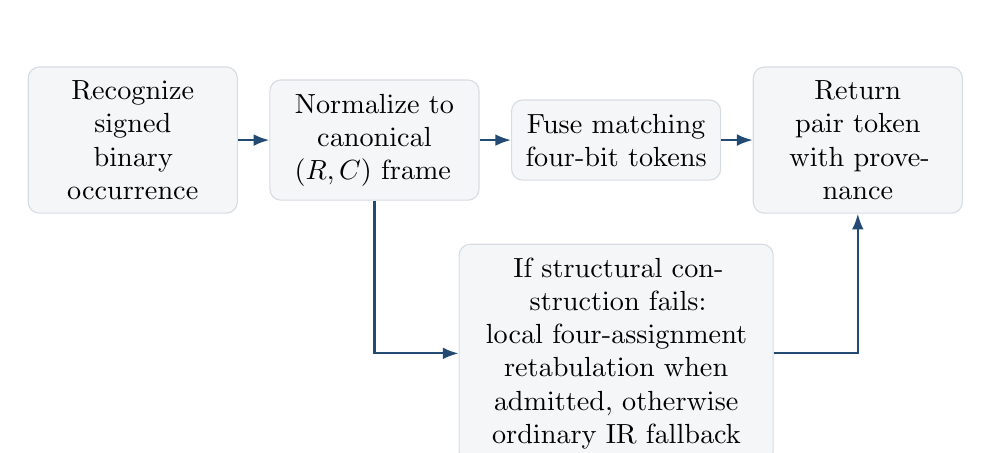
\begin{tikzpicture}[
 node distance=4mm and 4mm,
 box/.style={draw=rulegray,rounded corners,fill=soft,align=center,minimum height=10mm,text width=0.19\linewidth,inner sep=5pt},
 arrow/.style={-{Latex[length=2mm]},thick,draw=accent}
]
\node[box] (recognize) {Recognize signed\\binary occurrence};
\node[box,right=of recognize] (align) {Normalize to\\canonical $(R,C)$ frame};
\node[box,right=of align] (fuse) {Fuse matching\\four-bit tokens};
\node[box,right=of fuse] (out) {Return pair token\\with provenance};
\draw[arrow] (recognize)--(align);
\draw[arrow] (align)--(fuse);
\draw[arrow] (fuse)--(out);
\node[box,below=8mm of fuse,text width=0.30\linewidth] (fallback) {If structural construction fails:\\local four-assignment retabulation when admitted, otherwise ordinary IR fallback};
\draw[arrow] (align.south) |- (fallback.west);
\draw[arrow] (fallback.east) -| (out.south);
\end{tikzpicture}
\caption{The compiler transformation. The operation performed on the four-bit token is trivial; the semantic work is the typed recognition and normalization that determines when fusion is legal and what fallback is required.}
\label{fig:compiler-flow}
\end{figure}

\subsection{Why frame metadata matters}

Return to Equation~\eqref{eq:mismatch-expression}. The two implication tokens are numerically equal before typing, but the second occurrence's array coordinates refer to $(Y,X)$ rather than $(X,Y)$. Naively XORing the two unaligned arrays would return the zero token. Transposition moves the second operator into the target frame, after which Equation~\eqref{eq:mismatch-fold} correctly yields $[\bxor]$. The error is therefore not a deficiency of truth tables; it is a failure to track which assignment each stored bit denotes.

This distinction is closely related to established NPN-style input permutation/negation and output-negation operations \cite{Mishchenko2006,Zhou2019}. The present use is intentionally narrower than a general NPN canonicalizer. It treats frame transport as a local typing obligation for a particular rewrite.

\section{Pair compiler and soundness}
\label{sec:compiler}

\subsection{Judgment, invariant, and provenance}

Let expressions use the grammar
\begin{equation}
 e ::= Z\mid \neg e\mid e\,\Phi\,e,
 \label{eq:grammar}
\end{equation}
where $Z$ is a variable and $\Phi$ is one of the currently supported binary connectives AND, OR, XOR, implication, and equivalence. Fix distinct canonical variables $R$ and $C$ and a fixed-substitution map $F$ that binds neither variable on a returned pair path. Write $\Gamma=(R,C,F)$.

A typed pair result has judgment
\begin{equation}
 \Gamma\vdash e\Downarrow^p \Pair(R,C,t),
 \qquad p\in\{S,T,H\},
 \label{eq:judgment}
\end{equation}
with the intended invariant
\begin{equation}
 \eval_t(r,c)=e[r/R,c/C]
 \quad\text{for all }r,c\in\B,
 \label{eq:invariant}
\end{equation}
interpreted after the fixed substitutions in $F$.

Equation~\eqref{eq:judgment} can be read as follows: under compiler environment $\Gamma$, expression $e$ has been reduced to the four-bit token $t$ in canonical frame $(R,C)$, and $p$ records how that token was obtained. Equation~\eqref{eq:invariant} is the semantic contract. Each of the four token positions must return exactly the value of the original expression under the corresponding assignment to $R$ and $C$. The pair therefore carries both a compact Boolean function and the frame metadata needed to interpret its bit positions.

The provenance values are:
\begin{itemize}
 \item \textbf{$S$ --- structural:} the returned subtree used signed primitive recognition, token complement, and/or same-frame fusion only.
 \item \textbf{$T$ --- tabulated root:} the returned subtree itself was produced by evaluating all four assignments. The symbol $T$ avoids overloading $R$, which already denotes the row variable.
 \item \textbf{$H$ --- hybrid:} structural steps occur above at least one tabulated descendant.
\end{itemize}
A top-level compilation additionally records \texttt{ordinary\_fallback} when no pair judgment is derived.

\subsection{Rules, built up one step at a time}

The inference-rule bar is read as implication: if the premises above the bar hold, the compiler may derive the conclusion below it. The rules perform four conceptually distinct jobs: create a normalized primitive token, complement an already compiled token, fuse two already aligned tokens, and---when enabled---tabulate an exact two-variable subtree that structural recognition could not build.

\paragraph{Primitive normalization.}
Let $\ell_1,\ell_2$ be signed literals whose underlying variables are exactly $R$ and $C$ in either order. If the declared normalization procedure transports the primitive occurrence $\Theta(\ell_1,\ell_2)$ into the canonical frame and returns token $t$, then the compiler may derive
\[
\frac{
  \operatorname{Norm}_{\Gamma}(\Theta(\ell_1,\ell_2))=t
}{
  \Gamma\vdash \Theta(\ell_1,\ell_2)\Downarrow^S \Pair(R,C,t)
}.
\]
Normalization consists only of the declared operand exchange and row/column polarity transforms from Equation~\eqref{eq:input-transforms}. This is the structural base case: it establishes a token whose four bit positions already refer to the canonical assignments $(R,C)=(1,1),(1,0),(0,1),(0,0)$.

\paragraph{Negation: Equation~\eqref{eq:neg-rule}.}
Once a child has a correct token in the canonical frame, negating the expression requires only bitwise complement of that token:
\begin{equation}
\frac{\Gamma\vdash a\Downarrow^p\Pair(R,C,t_a)}
{\Gamma\vdash \neg a\Downarrow^{\nu(p)}\Pair(R,C,\neg t_a)}.
\label{eq:neg-rule}
\end{equation}
The frame does not change. Here $\neg t_a$ means complement each of the four token bits. Provenance changes only to report ancestry: $\nu(S)=S$ and $\nu(T)=\nu(H)=H$. Thus a structural NOT above a locally tabulated child is correct but explicitly reported as hybrid.

\paragraph{Same-frame fusion: Equation~\eqref{eq:fuse-rule}.}
Two compiled children may be fused only when their pair metadata name the same canonical frame:
\begin{equation}
\frac{\Gamma\vdash a\Downarrow^p\Pair(R,C,t_a)
\qquad
\Gamma\vdash b\Downarrow^q\Pair(R,C,t_b)}
{\Gamma\vdash a\Phi b\Downarrow^{p\sqcup q}\Pair(R,C,t_a\ptop{\Phi}t_b)}.
\label{eq:fuse-rule}
\end{equation}
The token operation $t_a\ptop{\Phi}t_b$ applies $\Phi$ independently to corresponding token positions. The repeated $\Pair(R,C,\cdot)$ in the two premises is the essential admission certificate: position $11$ in one child denotes the same assignment as position $11$ in the other, and similarly for $10,01,00$. Define $S\sqcup S=S$; every other combination is $H$ because tabulated ancestry is present below a structural fusion.

\paragraph{Exact local tabulation.}
When the selected strategy permits local tabulation and the live support after fixed substitution is exactly $\{R,C\}$, define the true-first token
\begin{equation}
 t_e:=\bigl(e(1,1),e(1,0),e(0,1),e(0,0)\bigr).
 \label{eq:tab-token}
\end{equation}
Then the exact tabulation rule is
\[
\frac{
  \supp_F(e)=\{R,C\}
  \qquad t=t_e
}{
  \Gamma\vdash e\Downarrow^T\Pair(R,C,t)
}.
\]
This rule re-evaluates a two-variable subtree on its complete four-assignment domain. It is therefore an exact fallback base case, not evidence that the compiler recognized the same structure syntactically.

\paragraph{Worked derivation.}
Let $\Gamma=(X,Y,\varnothing)$ and
\begin{equation}
 e=(X\Rightarrow\neg Y)\bxor(\neg Y\Rightarrow X).
 \label{eq:worked-expression}
\end{equation}
In true-first order $(11,10,01,00)$, implication has token $1011_2$. For the left child, the variables are already in $(X,Y)$ order but the column literal is negated, so the column-polarity transform gives
\[
 X\Rightarrow\neg Y\quad\longmapsto\quad 0111_2.
\]
For the right child, the source operands arrive as $(\neg Y,X)$. Operand exchange followed by polarity alignment gives
\[
 \neg Y\Rightarrow X\quad\longmapsto\quad 1110_2.
\]
Both children now carry frame $(X,Y)$, so Equation~\eqref{eq:fuse-rule} is legal:
\begin{equation}
 0111_2\ \bxor\ 1110_2=1001_2.
 \label{eq:worked-fusion}
\end{equation}
Hence
\[
 \Gamma\vdash e\Downarrow^S\Pair(X,Y,1001_2).
\]
The token $1001_2$ is $[\Leftrightarrow]$ in true-first order, so the compiler has established
\[
 (X\Rightarrow\neg Y)\bxor(\neg Y\Rightarrow X)=X\Leftrightarrow Y
\]
without first expanding the source expression into an ANF or another larger symbolic representation. Applying Equation~\eqref{eq:neg-rule} once more complements $1001_2$ to $0110_2$, the XOR token.

The public compiler strategies are therefore:
\begin{itemize}
 \item \textbf{\texttt{pure\_structural}:} primitive normalization, negation, and same-frame fusion only;
 \item \textbf{\texttt{hybrid}:} the structural rules plus exact local pair tabulation when needed;
 \item \textbf{\texttt{retabulate}:} bypass recursive pair construction and tabulate the whole admitted root;
 \item \textbf{ordinary fallback:} leave non-admitted expressions on the general IR path.
\end{itemize}
This explicit hybrid class is important. An earlier implementation/review cycle allowed a tabulated child to be consumed by a structurally compiled parent without naming that path. The current specification records it instead of silently treating it as purely structural.

\begin{theorem}[Pure structural soundness]
If $\Gamma\vdash e\Downarrow^S\Pair(R,C,t)$, then Equation~\eqref{eq:invariant} holds and no four-assignment tabulation was used.
\end{theorem}

\begin{proof}
Induct on the derivation. A signed primitive is correct by the frame transforms in Equation~\eqref{eq:input-transforms}; complementing a correct child represents negation; and fusing two correct children with identical metadata is sound by Theorem~1.
\end{proof}

\begin{definition}[Declared pure-structural fragment]
Fix canonical variables $R,C$. Let $\mathcal S_{R,C}$ be the smallest expression class containing every supported primitive $\Theta(\ell_1,\ell_2)$ whose signed literals have underlying variables exactly $R,C$ in either order, and closed under negation and the five supported binary connectives.
\end{definition}

\begin{theorem}[Completeness for the declared pure-structural fragment]
For every $e\in\mathcal S_{R,C}$, the \texttt{pure\_structural} strategy derives a unique canonical-frame token $t$ such that
\[
 \Gamma\vdash e\Downarrow^S\Pair(R,C,t)
\]
and Equation~\eqref{eq:invariant} holds.
\end{theorem}

\begin{proof}
Induct on the construction of $e$. Every primitive in $\mathcal S_{R,C}$ is admitted by primitive normalization. Negation preserves the frame and remains structural by Equation~\eqref{eq:neg-rule}. If two children belong to $\mathcal S_{R,C}$, induction gives tokens in the same canonical frame, so Equation~\eqref{eq:fuse-rule} applies. Uniqueness follows because a Boolean function on fixed variables $R,C$ has one four-bit truth token in the declared true-first order.
\end{proof}

\begin{remark}
This is syntactic completeness for the deliberately declared compiler fragment, not semantic completeness for all formulas with two-variable support. A semantically equivalent expression outside $\mathcal S_{R,C}$ may still require exact tabulation or ordinary fallback.
\end{remark}

\begin{lemma}[Exact pair tabulation]
Suppose the live support after fixed substitution is exactly one distinct row variable $R$ and one distinct column variable $C$. Evaluating $e$ at $(1,1),(1,0),(0,1),(0,0)$ and storing those four outputs in true-first order produces the unique token satisfying Equation~\eqref{eq:invariant}.
\end{lemma}

\begin{theorem}[Soundness of admitted pair compilation]
Every derivable pair result with provenance $p\in\{S,T,H\}$ satisfies Equation~\eqref{eq:invariant}. If no pair judgment is derivable, correctness is delegated to the unchanged ordinary IR evaluator.
\end{theorem}

\begin{proof}
The cases $S$ and $T$ are the preceding theorem and lemma. For $H$, use structural induction with exact local tabulation as an additional sound base case; token complement and same-frame fusion preserve the invariant. Provenance changes the reported construction path, not the represented function. The fallback statement is an interface contract rather than a theorem about the pair compiler itself.
\end{proof}

\subsection{Admissibility boundary}

The current pure structural rule does not claim semantic recognition of arbitrary equivalent compound operands. Repeated-variable forms such as $X\Theta X$, overlapping row/column layouts, opaque compound operands, and different variable pairs remain outside the pure rule. A retabulation rule may cover some two-variable cases exactly, but it is intentionally classified as a different mechanism.

This conservative boundary is useful. It allows the compiler to refuse a local rewrite rather than infer an unproved equivalence. It also gives the experiment a measurable fallback frequency instead of hiding unsupported cases in preprocessing.

\section{Implementation architecture and cost model}
\label{sec:implementation}

\subsection{Five artifacts, not one}

Table~\ref{tab:artifacts} separates implementation objects that are easily conflated when all are described informally as a ``CM.''

\begin{table}[t]
\centering
\small
\begin{tabularx}{\linewidth}{@{}p{0.18\linewidth}X p{0.21\linewidth}@{}}
\toprule
\textbf{Artifact} & \textbf{Meaning} & \textbf{Role}\\
\midrule
CM operator token & One binary truth function packed into four true-first bits $(11,10,01,00)$. & Constant-size transform and fusion.\\
Pair surrogate & Token plus canonical row and column operand names/frame metadata. & Carries the legality invariant.\\
General CM/Boolean IR & Interned expression DAG for arbitrary supported formulas. & General symbolic fallback and compilation.\\
Flat program & Backend-dependent instruction sequence lowered from the IR. & Repeated packed/array evaluation.\\
Explicit dense output & Materialized truth relation over requested unfixed Boolean axes. & User-visible output; $2^n$ bits for $n$ axes.\\
\bottomrule
\end{tabularx}
\caption{Compiler artifacts and their semantic boundaries. Only the first is the constant-size binary operator token.}
\label{tab:artifacts}
\end{table}

A token-only endpoint cannot be compared as if it had already paid to construct an explicit $2^n$-entry result. Conversely, a comparator that has already prepared a reusable DAG or program should not be charged for that preparation on every query when the CM arm is allowed resident reuse. Endpoint equality is part of benchmark correctness.

\subsection{Executable case ordering}

The implementation logic can be summarized as follows.

\begin{lstlisting}
Pair(node e, frame Gamma, bool allowRetab):
    if e is a supported binary connective over signed literals:
        recognize row/column variables and finite negation chains
        normalize operand order and polarity into Gamma
        return structural Pair(R, C, token)

    if e = NOT a and Pair(a, Gamma, allowRetab) succeeds:
        complement token; preserve/upgrade provenance
        return Pair(...)

    if e = a Phi b and both recursive Pair calls succeed
       with identical canonical (R,C) metadata:
        fuse tokens entrywise under Phi
        return Pair(...)

    if allowRetab and live_support(e after fixed substitutions) = {R,C}:
        evaluate e on (1,1),(1,0),(0,1),(0,0)
        return retabulated Pair(R,C,token)

    return no-pair

TopLevel(e, strategy):
    pure_structural -> Pair(..., allowRetab=false) or ordinary IR
    hybrid          -> Pair(..., allowRetab=true)  or ordinary IR
    retabulate      -> exact whole-root four-assignment token if admitted
\end{lstlisting}

Every recursive pair call receives a strict AST child, so structural recursion terminates on finite expressions. Retabulation performs four finite evaluations.

\subsection{Layout conversion and ownership}

The compact token uses true-first order while the historical dense array path uses false-first axes. The conversion is an explicit reindexing. If $T$ denotes the true-first $2\times2$ view and $D$ the false-first view indexed by array positions $a,b\in\{0,1\}$, then
\begin{equation}
 D_{ab}=T_{1-a,1-b}.
 \label{eq:layout-conversion}
\end{equation}
Axes absent from the compact pair can then be broadcast into the requested output layout. The materialized dense result must be an owned output rather than a writable broadcast view. Expression nodes and pair surrogates are immutable under the compiler contract, and caller-owned layouts/fixed maps are read-only.

\subsection{Cost model}

Let $N$ be AST occurrences, $U$ unique DAG nodes, $H$ AST height, $S$ occurrences in a subtree sent to retabulation, $D$ its evaluation depth, $k$ the length of a signed literal's negation chain, and $n$ the number of requested unfixed output axes.

\begin{itemize}
 \item Inspecting a signed literal costs $O(k)$ followed by an $O(1)$ four-bit transform.
 \item A four-bit token fusion is $O(1)$.
 \item One exact pair retabulation costs $O(4S)$ time plus the evaluator's stack/workspace requirements.
 \item A fully successful structural pair tree is ordinarily $O(N)$ time and $O(H)$ stack space, although the current support-discovery strategy can rescan rejected subtrees and therefore has an $O(N^2)$ worst case.
 \item A sharing-aware evaluator may scale with $U$ rather than $N$, which is why DAG-preserving packed/CSE comparators are mandatory.
 \item Materializing an arbitrary complete output over $n$ unfixed Boolean axes costs $\Theta(2^n)$ time and output space for every explicit method.
\end{itemize}

The last point prevents a common category error: constant-time token fusion is a local kernel fact, not an end-to-end complexity theorem.

\section{Closest prior art and matched comparators}
\label{sec:related}

The compiler should be compared with operations that possess equivalent local information, not with deliberately weaker baselines.

\paragraph{Boolean matrices and truth vectors.}
Edwards developed Boolean-matrix logic well before the present work \cite{Edwards1972}. Cheng, Zhao, and Xu use XOR as addition and AND as multiplication and state an entrywise outer-operation law on truth vectors of the same ordered variables \cite{Cheng2011}. Reshaping such a vector into $2\times2$ form does not make that pointwise identity new.

\paragraph{Matrix/vector logic.}
Stern and Mizraji provide established operator/matrix representations of logic \cite{Stern1988,Mizraji1992,Mizraji2008}. Bricken's technical note explicitly places logical matrices between two-component states in bra--matrix--ket form \cite{Bricken1997}. The companion foundations paper contains the appropriate broader comparison; the computational manuscript needs only enough of this history to prevent novelty from being attached to notation or representation alone.

\paragraph{NPN, LUT, and AIG practice.}
Small truth functions are routinely packed into machine words, transformed under input permutation/negation and output negation, classified up to NPN equivalence, and used in cut-based rewriting. DAG-aware AIG rewriting specifically exploits graph sharing rather than treating a formula as an unshared tree \cite{Mishchenko2006,Zhou2019,Testa2019}. CM transposition, row/column reversal, complement, and four-bit storage are therefore best understood as a particular typed use of familiar small-function operations.

\paragraph{Direct packed evaluation.}
A strong simple comparator evaluates the AST once over four packed masks to obtain all four assignments in parallel. With identity memoization it also preserves explicit DAG sharing. It returns exactly the same four-bit function required by a pair-token endpoint and does not need CM-specific frame metadata. This is the closest baseline for deciding whether structural recognition pays for itself.

\paragraph{Generic local truth-function optimization.}
A generic optimizer given the same local support/function information can tabulate or combine a small cut without using CM notation. The S1/S2 evidence below shows why this comparator is scientifically necessary: it reaches the same reduced symbolic outputs as CM folding on the admitted all-arm cases.

\paragraph{ROBDDs and broader rewrite search.}
ROBDDs provide canonical function representations for a fixed variable order \cite{Bryant1986}. Equality saturation and synthesis-driven superoptimization retain or search broader classes of equivalent expressions \cite{Willsey2021,Sasnauskas2017}. These systems solve a more general problem than the fixed two-operand rule; comparison should therefore charge recognition/search/extraction and compare delivered artifacts appropriate to the task.

\section{Experimental questions and evidence hierarchy}
\label{sec:evaluation}

The computational claim is meaningful only if the benchmark answers the same question for every arm. Four distinctions are especially important.

\begin{enumerate}
 \item \textbf{Kernel versus compiler.} Four-bit fusion time is not compilation time.
 \item \textbf{Prepared versus one-shot.} A resident token/program may amortize setup; one-shot use may not.
 \item \textbf{Compact versus materialized output.} A token endpoint is not a complete $2^n$ truth relation.
 \item \textbf{Task contract.} ANF production, complete truth-vector evaluation, repeated restriction, counting, and multi-root output are different tasks and cannot share one headline ratio.
\end{enumerate}

Figure~\ref{fig:evidence-levels} shows the evidence levels used in this draft.

\begin{figure}[H]
\centering
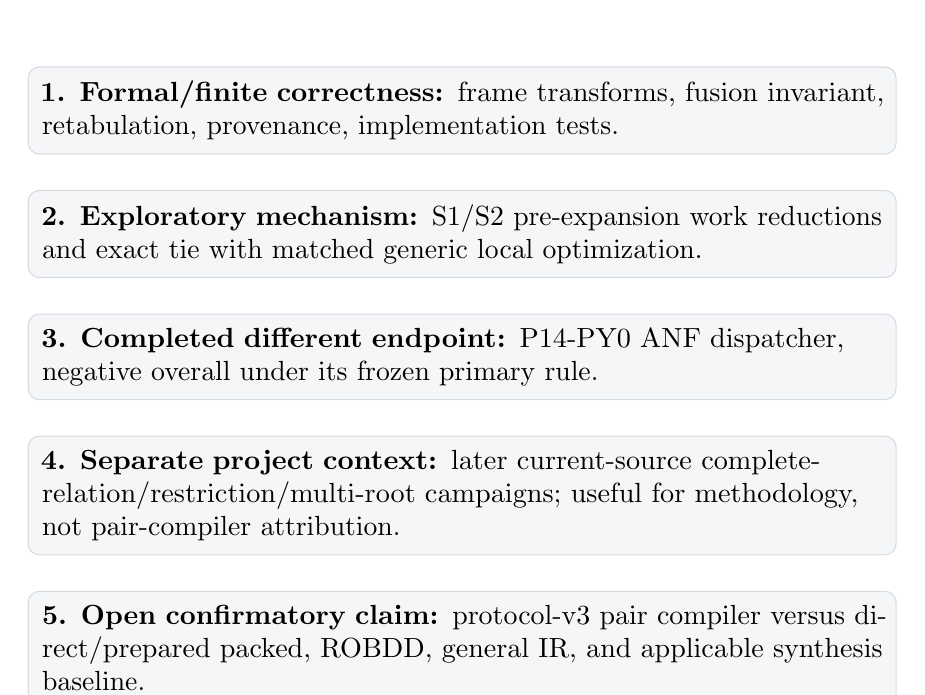
\begin{tikzpicture}[
 node distance=4.5mm,
 level/.style={draw=rulegray,rounded corners,fill=soft,align=left,text width=0.88\linewidth,inner sep=5pt},
]
\node[level] (a) {\textbf{1. Formal/finite correctness:} frame transforms, fusion invariant, retabulation, provenance, implementation tests.};
\node[level,below=of a] (b) {\textbf{2. Exploratory mechanism:} S1/S2 pre-expansion work reductions and exact tie with matched generic local optimization.};
\node[level,below=of b] (c) {\textbf{3. Completed different endpoint:} P14-PY0 ANF dispatcher, negative overall under its frozen primary rule.};
\node[level,below=of c] (d) {\textbf{4. Separate project context:} later current-source complete-relation/restriction/multi-root campaigns; useful for methodology, not pair-compiler attribution.};
\node[level,below=of d] (e) {\textbf{5. Open confirmatory claim:} protocol-v3 pair compiler versus direct/prepared packed, ROBDD, general IR, and applicable synthesis baseline.};
\end{tikzpicture}
\caption{Evidence hierarchy. A favorable result on a different endpoint is not promoted into pair-compiler evidence.}
\label{fig:evidence-levels}
\end{figure}

\subsection{Confirmatory workload design}

Protocol v3 separates exact-frame formulas, signed/swapped frames, local retabulation cases, hybrid mixed-child cases, multiple operand pairs, compound-operand cases outside the structural claim, and natural formulas/circuits. Balanced generated trees use AST occurrence counts $15,63,255,1023,4095$; skewed trees stop at 255 occurrences and measured height at most 128. Cases cross the five supported outer connectives, reuse counts $1,10,100,1000$, and sharing conditions that distinguish identity-shared nodes, structurally equal but separately allocated subtrees, and no sharing. Every case records both $N$ and $U$.

Requested outputs include compact tokens, scalar evaluation, packed batches, and dense outputs where the output budget permits them. Preparation and query costs are reported separately. Once two arms have produced the same four-bit token and call the same lookup function, the query cost is common; any advantage must arise earlier or through a measured reuse policy.

The sole primary cell is intentionally narrow: signed/permuted pure-structural balanced formulas with $N=1023$, $U=N$, no fixed variables, token output, reuse one, compared end to end with direct packed AST evaluation. The preregistered success rule requires zero correctness disagreements, a median competitor-to-CM ratio of at least $1.20$ whose 95\% interval lies entirely above one, and no more than a 10\% median peak-memory increase. All other cells are secondary. This prevents a favorable post hoc workload from replacing a failed primary comparison.

\section{Current evidence}
\label{sec:results}

\subsection{Correctness and implementation assurance}

The current implementation record reports 116 focused tests passing in an isolated source-copy run on 19 September 2026. The tested surface includes all 16 tokens in eight signed operand frames, the five supported primitive connectives, recursive fusion after alignment, pure-versus-hybrid provenance, whole-root retabulation, fixed substitutions in the direct packed comparator, true-first constants, 250 seeded random two-variable formulas, token-only API behavior, output-budget behavior, and input nonmutation. A separate exhaustive check enumerates 1,048,576 signed-alignment/fusion cases.

These counts are implementation assurance, not proofs of unbounded theorems and not evidence of speed. For submission, the test output, source hash, command, and environment should be bound into the same archival evidence package as the manuscript.

\subsection{S1/S2: mechanism evidence and the generic tie}

The canonical exploratory S1/S2 record contains 10,500 generated cases. Of these, 10,389 completed in all four arms: direct ANF, sharing-aware common-subexpression evaluation, a generic local truth-function optimizer, and CM folding. The all-arm population contains 3,750 S1 and 6,639 S2 cases. The remaining 111 are retained rather than silently filtered: 108 fail in all arms, two complete only in the generic and CM arms, and one only in the sharing arm. No completed correctness disagreement was recorded.

On every admitted all-arm case, CM and generic local optimization agree on seven principal symbolic-output metrics: final degree, final monomial count, multiplication count, output unique nodes, pair terms, peak monomials, and serialized bytes. The generic arm records more folds on 6,010 cases and CM more on none; fold count is not runtime. For corrected S2, median direct/CM multiplication counts at requested sharing fractions $0$, $0.25$, and $0.5$ are respectively $35/35$, $17/12$, and $9/0$.

The correct interpretation is therefore two-sided. Local small-function folding can remove work before polynomial expansion in some structures. The observed reduction is not uniquely CM-specific: an equally capable generic local optimizer reaches the same reduced outputs. This is mechanism evidence, not an end-to-end speed result.

\subsection{P14-PY0: a completed negative dispatcher boundary}

P14-PY0 measures a different endpoint: recipe-to-owned-ANF compilation. Direct lowering (D) lowers the ordinary source DAG; a minimal observer (F) records dispatch information; exact dispatch (E) decides whether to lower directly or construct folding metadata; always-fold (A) and a generic signature optimizer (G) are diagnostics. Preparation required by an arm is included in its production timer. This is not the direct packed token task of protocol v3.

The frozen campaign used 384 synthetic cases from 12 families and 107 natural cones from 14 previously uninspected EPFL design families, for 491 frozen cases. Three fresh sequential workers produced 51,102 measured rows including diagnostics/canonicalization; equality checks passed the 491 frozen cases and 512 targeted correctness cases. Exact dispatch selected folding on five synthetic cases and no natural cone.

\begin{table}[t]
\centering
\small
\begin{tabular}{@{}llcc@{}}
\toprule
\textbf{Corpus} & \textbf{Ratio} & \textbf{Geometric mean} & \textbf{98.75\% simultaneous interval}\\
\midrule
Synthetic & E/F & 0.9606 & [0.9455, 0.9811]\\
Synthetic & E/D & 1.0508 & [0.9683, 1.1075]\\
Natural & E/F & 0.9610 & [0.9411, 1.0001]\\
Natural & E/D & 1.0607 & [1.0176, 1.0927]\\
\bottomrule
\end{tabular}
\caption{Frozen P14-PY0 recipe endpoint. Ratios below one favor the numerator.}
\label{tab:p14}
\end{table}

The frozen primary rule required E/F geometric mean at most 0.99, E/D at most 0.95, and the relevant simultaneous upper bound below one on both corpora. It did not pass. At this endpoint exact dispatch was about 5.1\% slower than direct lowering on the synthetic corpus and 6.1\% slower on the natural corpus. The five selected synthetic cases themselves were highly profitable, with E/D ratios between 0.075 and 0.389, but those local wins did not offset aggregate policy overhead. The preregistered case-balanced geometric mean is retained even though an alternative ratio of summed synthetic medians was favorable. This is precisely the sort of negative boundary a selective compiler paper should report.

\subsection{Later project-wide results: relevant context, different contracts}
\label{sec:later-context}

The broader public CM project continued benchmarking after the manuscript snapshot. Two later records are especially relevant to interpretation, but neither measures the protocol-v3 pair compiler.

First, a 25 August 2026 audit correction strengthened the generic comparator on a post-compilation kernel study. On its matched successor, sharing-aware CSE-flat and bare CM both reduced work relative to raw-AST execution. The formula-balanced bare-CM/CSE-flat ratio was 0.891 overall, narrowing to 0.961 at live support $k=16$, while the public CM wrapper remained slower (2.797$\times$ CSE-flat overall and 1.343$\times$ at $k=16$) \cite{ProjectCorrection20260825}. The project therefore distinguishes a favorable kernel boundary from an unfavorable one-shot wrapper boundary.

Second, a source-closed architecture comparison completed on 3--4 September 2026. For a complete explicit-relation task, a packed CM-IR arm was 1.053$\times$ faster than dense CM but achieved only 0.930$\times$ against the current identity-memoized direct BitSet arm; BitSet won all 78 runnable case clusters. In the corrected q1/q4/q16/q64 repeated-restriction ladder, Python R2 led at q1/q4 and CSE-flat bigint led at q16/q64 on the first host; at q64 CSE-flat was 1.100$\times$ over R2, won all 54 cases, and retained a minimum above one. A separate host/compiler replication preserved the q1/q4 and q64 ordering, with CSE-flat at 1.090$\times$ over R2 at q64. Native fused slots showed aggregate gains in some cohorts but unfavorable minima and remained guarded rather than universal defaults \cite{ProjectArchitecture20260903}.

These later campaigns strengthen three methodological choices in the present paper: use direct packed evaluation as a first-class comparator, measure preparation/reuse explicitly, and keep task contracts separate. They do \emph{not} fill the protocol-v3 pair-compiler result table.

\subsection{The confirmatory gap}

The broader token/packed protocol v3 remains unexecuted in the current manuscript record. Until that campaign is frozen and run, the paper cannot answer the strongest end-to-end question: whether typed structural recognition and frame normalization repay their costs against an equivalently capable direct packed/DAG baseline on the primary workload.

This gap is not hidden by substituting S1/S2, P14-PY0, or later project-wide architecture runs. Each of those records answers a different question.

\section{Discussion}
\label{sec:discussion}

\subsection{What the CM representation specifically contributes}

The raw four truth values are not new. The computationally useful structure is the combination of a compact token with an explicit frame. That representation provides four practical properties.

First, \emph{legality is local}: equality of canonical row/column metadata is a direct certificate for same-frame fusion. Second, signed normalization is fixed and cheap after recognition: transpose and row/column swaps act directly on four bits. Third, the fused result remains another four-bit token in the same frame, so the rewrite composes without expanding the operands. Fourth, provenance can say whether the token was derived structurally, retabulated, or assembled from both mechanisms.

A generic optimizer can implement the same semantic reduction with a different representation. The question is therefore not whether CM has exclusive access to the reduction, but whether the CM/frame organization lowers the engineering cost of recognizing and composing it in a larger compiler.

\subsection{When folding can help}

Folding is most plausible when the same two live operands recur through multiple signed/order variants, when expansion would otherwise repeat symbolic work, when the result will be reused, or when a local cut can be collapsed before an expensive downstream representation is built. The S1/S2 sharing strata provide a direct illustration: the largest observed reductions occur where repeated/local structure gives the small-function rewrite something to eliminate.

The same mechanism becomes less attractive when compatible pairs are rare, support discovery rescans rejected subtrees, a sharing-aware baseline evaluates unique DAG nodes once, a one-shot call cannot amortize preparation, or the requested output forces a much larger materialization. The later project-wide wrapper and BitSet results show that these overheads are not theoretical nuisances; they can dominate otherwise favorable kernel operations.

\subsection{Retabulation is useful but conceptually different}

Evaluating four assignments is exact for a two-variable function, but it should not be allowed to make a structural recognition rule look more powerful than it is. Retabulation consumes the subtree as a black box and reconstructs its local truth function. Structural folding instead proves that a token can be derived compositionally from recognized children and frame transforms. Both are valid compiler techniques; their costs and explanatory value differ.

This is why the hybrid path has its own provenance. It allows the practical compiler to continue after a local retabulation while preserving an auditable distinction between recognition and re-evaluation.

\subsection{Sharing and output type change the break-even point}

An AST occurrence count can dramatically overstate work when a comparator preserves identity sharing. Reporting both $N$ and $U$ is therefore mandatory. Equal-but-separately-allocated subtrees must also be distinguished from identity-shared nodes because hash-consing or structural CSE may discover the former while simple identity memoization does not.

Output type matters just as much. A four-bit token is a legitimate endpoint for a small-function compiler decision; it is not equivalent to returning a dense relation over many variables. Conversely, if a caller asks for repeated scalar or residual queries, preserving a prepared compact representation may be more important than materializing the full vector. Break-even reuse should therefore be derived from measured setup and per-query costs, not from an isolated token-fusion benchmark.

\subsection{What a negative protocol-v3 result would mean}

A negative confirmatory result would not invalidate the soundness theorem or the observation that local folding can reduce symbolic work. It would show that, under the tested implementation and workload distribution, recognition/planning/fallback costs erase those reductions relative to strong generic methods. That is a scientifically coherent outcome and would sharpen the contribution into a compiler-mechanism and evaluation-boundary paper.

Conversely, a positive result should remain scoped to the exact output, reuse, sharing, and workload region that passes the frozen rule. The later architecture campaigns demonstrate why a task map is more informative than a universal ratio.

\section{Limitations}

The current compiler intentionally recognizes a narrow class of two-operand local structure. It does not solve general Boolean equivalence, NPN canonicalization, LUT mapping, AIG rewriting, or broad superoptimization. Its support-discovery implementation can have a quadratic worst case on rejected structures. The implementation uses a host-language recursive traversal and therefore imposes an explicit height bound on skewed benchmark cells rather than relying on an increased recursion limit.

The S1/S2 corpus is synthetic/exploratory and contains only sixteen possible semantic functions on a fixed two-variable support; large two-variable trees measure syntactic redundancy and compiler behavior rather than growing semantic complexity. P14-PY0 measures ANF lowering rather than the packed-token endpoint. The later August/September project records use still other task contracts. Natural-workload prevalence of pure structural pair folding remains unresolved for this paper.

Finally, an explicit truth relation over $n$ unfixed variables contains $2^n$ outputs. CM layout does not remove that information-theoretic output size. Compression, symbolic sharing, and partial-query benefits must be evaluated as separate representation or task properties.

\section{Conclusion}

The computational role of correspondence matrices is most defensible when stated narrowly. A four-bit binary operator token becomes useful to a compiler when its operand frame is typed. Signed and swapped occurrences can then be transported to a canonical frame, compatible tokens can be fused before operand evaluation or expansion, and unsupported structures can be retabulated or returned to an ordinary IR without compromising correctness.

The existing evidence draws an equally important boundary. Local small-function folding can reduce pre-expansion work, but a matched generic optimizer can reproduce the same symbolic reductions. A frozen dispatcher campaign shows that even very profitable local choices can lose overall once decision overhead is charged. Later project-wide benchmarks reinforce the need for direct packed/CSE baselines and task-matched endpoints, but they are not substitutes for the unexecuted pair-compiler protocol.

The next empirical question is therefore precise: on what workload, output, sharing, and reuse regimes does the typed frame-aware compiler repay its recognition and preparation costs? A completed protocol-v3 campaign can answer that question without requiring any claim that the underlying truth-table operations are uniquely CM-specific.

\appendix

\section{Compact proof details}

\subsection{Signed transformations}

Left multiplication by $P$ exchanges the two rows of $[\Theta]$, so the row-$x$, column-$y$ entry becomes the original row-$\neg x$, column-$y$ entry, which is $(\neg x)\Theta y$. Right multiplication exchanges columns. Transposition exchanges the two assignments. Because $P$ is a permutation matrix under XOR--AND multiplication, no multi-term cancellation occurs in these reindexings.

\subsection{Hybrid induction}

For pure structural derivations, primitive normalization is the base case and Equations~\eqref{eq:neg-rule}--\eqref{eq:fuse-rule} preserve Equation~\eqref{eq:invariant}. For a hybrid derivation, exact local tabulation supplies an additional sound base case. Every parent above that base is again token complement or same-frame fusion. Thus hybrid provenance records how the token was obtained but does not alter its denotation.

\subsection{Uniqueness of tabulated token}

Fix $R,C$. Any binary Boolean function on those two variables is determined by its four values on $(1,1),(1,0),(0,1),(0,0)$. Storing those values in the declared true-first token order therefore produces the unique token that agrees with the source expression on every assignment.

\section{Current verification scope and submission checklist}

The current manuscript/review artifacts report a focused 116-test run and an independent exhaustive signed-alignment/fusion enumeration of 1,048,576 cases. Before submission these should be re-executed from the same content-addressed source snapshot used for the final benchmark. The archival package should include the exact commands and stdout, source/environment hashes, natural-corpus provenance, raw S1/S2 and P14-PY0 records, protocol-v3 freeze and raw observations, ABC/AIG tool configuration for its admitted subset, analysis scripts, failures/timeouts, and a public archive identifier.

\begin{thebibliography}{99}

\bibitem{Bricken1997}
William Bricken.
\newblock \emph{Notes on Matrix Techniques for Logic}.
\newblock Technical note internally dated March 1997; original public-release date and peer-reviewed status not established.
\newblock \url{https://wbricken.com/pdfs/01bm/01math/03math-supporting/math-tangential/04matrix-tech.pdf}.

\bibitem{Bryant1986}
Randal E. Bryant.
\newblock Graph-based algorithms for Boolean function manipulation.
\newblock \emph{IEEE Transactions on Computers}, C-35(8):677--691, 1986.
\newblock doi:10.1109/TC.1986.1676819.

\bibitem{Cheng2011}
Daizhan Cheng, Yin Zhao, and Xiangru Xu.
\newblock Matrix approach to Boolean calculus.
\newblock In \emph{Proceedings of the 50th IEEE Conference on Decision and Control and European Control Conference}, pages 6950--6955, 2011.
\newblock doi:10.1109/CDC.2011.6160289.

\bibitem{Droncheff2018}
Brian Droncheff.
\newblock \emph{Correspondence Matrices; Algorithms for Propositional Logic}.
\newblock ResearchGate preprint, 2018.
\newblock doi:10.13140/RG.2.2.28036.37764.

\bibitem{Edwards1972}
C. R. Edwards.
\newblock The logic of Boolean matrices.
\newblock \emph{The Computer Journal}, 15(3):247--253, 1972.
\newblock doi:10.1093/comjnl/15.3.247.

\bibitem{Lee2022}
Winston Lee, Heinz Riener, Alan Mishchenko, Robert K. Brayton, and Giovanni De Micheli.
\newblock A simulation-guided paradigm for logic synthesis and verification.
\newblock \emph{IEEE Transactions on Computer-Aided Design of Integrated Circuits and Systems}, 41(8):2573--2586, 2022.
\newblock doi:10.1109/TCAD.2021.3108704.

\bibitem{Mishchenko2006}
Alan Mishchenko, Satrajit Chatterjee, and Robert K. Brayton.
\newblock DAG-aware AIG rewriting: A fresh look at combinational logic synthesis.
\newblock In \emph{Proceedings of the 43rd Design Automation Conference}, pages 532--536, 2006.
\newblock doi:10.1145/1146909.1147048.

\bibitem{Mizraji1992}
Eduardo Mizraji.
\newblock Vector logics: The matrix--vector representation of logical calculus.
\newblock \emph{Fuzzy Sets and Systems}, 50(2):179--185, 1992.
\newblock doi:10.1016/0165-0114(92)90216-Q.

\bibitem{Mizraji2008}
Eduardo Mizraji.
\newblock Vector logic: A natural algebraic representation of the fundamental logical gates.
\newblock \emph{Journal of Logic and Computation}, 18(1):97--121, 2008.
\newblock doi:10.1093/logcom/exm057.

\bibitem{ProjectCorrection20260825}
Correspondence Matrices Project.
\newblock \emph{CM benchmark audit correction --- 2026-08-25}.
\newblock Public technical record, 25 August 2026.
\newblock \url{https://github.com/Relative0/Correspondence_Matrices/blob/main/deliverables_n22_24/corrections_2026_08_25/CM_BENCHMARK_AUDIT_CORRECTION_REPORT_2026-08-25.md}.

\bibitem{ProjectArchitecture20260903}
Correspondence Matrices Project.
\newblock \emph{Architecture-aware CM comparison refresh after C37}.
\newblock Public technical record, 3 September 2026; updated 4 September 2026.
\newblock \url{https://github.com/Relative0/Correspondence_Matrices/blob/main/docs/research/CM_ARCHITECTURE_AWARE_COMPARISON_REFRESH_AFTER_C37_2026_09_03.md}.

\bibitem{Sasnauskas2017}
Raimondas Sasnauskas et al.
\newblock Souper: A synthesizing superoptimizer.
\newblock arXiv:1711.04422, 2017.

\bibitem{Stern1988}
August Stern.
\newblock \emph{Matrix Logic: Theory and Applications}.
\newblock North-Holland, 1988.

\bibitem{Testa2019}
Eleonora Testa, Mathias Soeken, Luca Gaetano Amar\`u, and Giovanni De Micheli.
\newblock Logic synthesis for established and emerging computing.
\newblock \emph{Proceedings of the IEEE}, 107(1):165--184, 2019.
\newblock doi:10.1109/JPROC.2018.2869760.

\bibitem{TheoryFoundations2026}
Brian Theory.
\newblock \emph{Correspondence and Logical Matrices: A Boolean Operator Calculus: Formula-valued logical matrices, valuation, pairing, and coherent operator superposition}.
\newblock Companion research draft, 22 September 2026.

\bibitem{Willsey2021}
Max Willsey, Chandrakana Nandi, Yisu Remy Wang, Oliver Flatt, Zachary Tatlock, and Pavel Panchekha.
\newblock egg: Fast and extensible equality saturation.
\newblock \emph{Proceedings of the ACM on Programming Languages} (POPL), 2021.
\newblock arXiv:2004.03082.

\bibitem{Zhou2019}
Xuegong Zhou, Lingli Wang, and Alan Mishchenko.
\newblock Fast adjustable NPN classification using generalized symmetries.
\newblock \emph{ACM Transactions on Reconfigurable Technology and Systems}, 12(2):7, 2019.
\newblock doi:10.1145/3313917.

\end{thebibliography}

\end{document}
